\chapter{Pre-Class}
\section{Number Fields}
\begin{defn}
A field is any set $\K$ which follow the Field Axioms:
\begin{enumerate}
   \item $\alpha + \beta = \beta + \alpha$ (addition is commutative).
   \item $(\alpha + \beta) + \gamma =\alpha + (\beta + \gamma)$ (addition is associative).
   \item There exists an element $0$ such that $\alpha + 0 = \alpha$.
   \item For every $\alpha \in \K$, there exists $\beta$ such that $\alpha + \beta = 0$.
   \item $\alpha\beta = \beta\alpha$ (multiplication is commutative).
   \item $(\alpha\beta)\gamma = \alpha(\beta\gamma)$ (multiplication is associative).
   \item There exists an element $1$ such that $1\cdot \alpha = \alpha$.
   \item For every $\alpha$ there exists a $\gamma$ such that $\alpha\gamma = 1$.
   \item $\alpha(\beta + \gamma) = \alpha\beta + \alpha\gamma$, multiplication is distributive over addition.
\end{enumerate}
\end{defn}
\begin{defn}
Two fields, $\K$ and $\K'$ are said to be \textbf{isomorphic} if we can setup a one to one correspondence between $\K$ and $\K'$.
\end{defn}
The most common fields are, $\Q$, $\R$, $\C$.

\section{Theory of Linear Algebra}
Involving space, and the most general case, a series of linear equations.
\[a_{11}x_{11} + a_{12}x_{12} + \dots + a_{1n}x_{1n} = b_1\]
\[a_{21}x_{21} + a_{22}x_{22} + \dots + a_{2n}x_{2n} = b_2\]
\[\dots \dots \dots \dots \dots \dots \dots \dots \dots\]
\[a_{n1}x_{n1} + a_{n2}x_{n2} + \dots + a_{nn}x_{nn} = b_n\]

\section{Determinant}
The determinant is the scalar that a 1 area, volume, hypervolume etc. gets scaled by. Even a one length can be scaled or reduced to 0. When a determinant is 0, it means that all space, gets squished to a lower dimension and thus has 0 volume, or 0 area, and so on.
\[D = 
\begin{vmatrix}
a_{11} & a_{12} & \dots & a_{1n}\\
a_{21} & a_{22} & \dots & a_{2n}\\
\vdots & \vdots & \ddots & \vdots \\
a_{n1} & a_{2n} & \dots & a_{nn}
\end{vmatrix} = \det||a||
\]

\begin{figure}
  \centering
  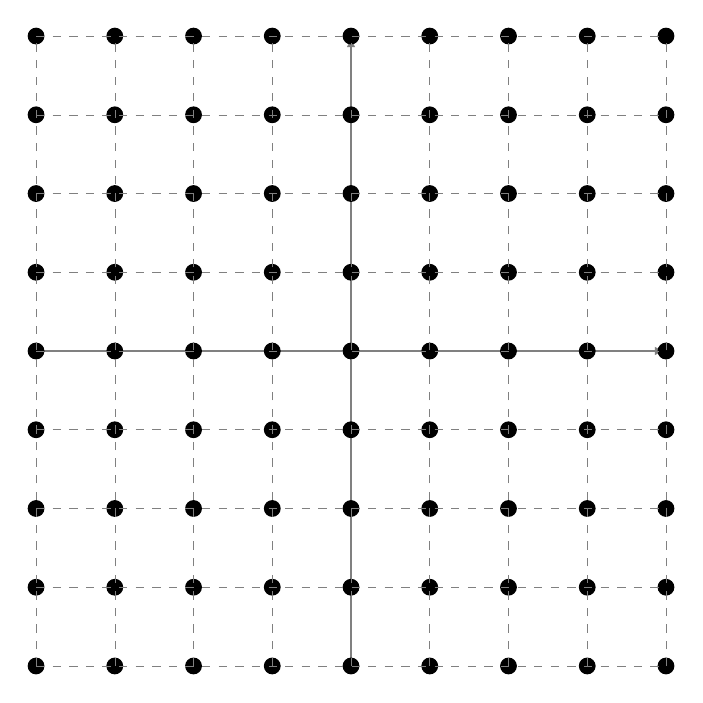
\begin{tikzpicture}[scale=1]
    \coordinate (Origin)   at (0,0);
    \coordinate (XAxisMin) at (-4,0);
    \coordinate (XAxisMax) at (4,0);
    \coordinate (YAxisMin) at (0,-4);
    \coordinate (YAxisMax) at (0, 4);
    \draw [thin, gray,-latex] (XAxisMin) -- (XAxisMax);% Draw x axis
    \draw [thin, gray,-latex] (YAxisMin) -- (YAxisMax);% Draw y axis

    %\clip (-3,-2) rectangle (10cm,10cm); % Clips the picture...
    \pgftransformcm{1}{0}{0}{1}{\pgfpoint{0cm}{0cm}}
          % This is actually the transformation matrix entries that
          % gives the slanted unit vectors. You might check it on
           % MATLAB etc. . I got it by guessing.
          % Draws a grid in the new coordinates.
    \foreach \x in {-4,-3,...,4}{% Two indices running over each
      \foreach \y in {-4,-3,...,4}{% node on the grid we have drawn 
        \node[draw,circle,inner sep=2pt,fill] at (\x,\y) {};
            % Places a dot at those points
      }
    }
    \draw[style=help lines,dashed] (-4,-4) grid[] (4,4);
  \end{tikzpicture}
  \caption{Vector Space $\R^2$ for $\forall (x,y); -4 \leq x \leq 4 and -4 \leq y \leq 4$.}
  \label{figure:solving-CVP-bad-basis}
\end{figure}

